\documentclass[tikz,border=10pt]{standalone}
\usepackage{amsmath}
\usetikzlibrary{arrows.meta,positioning,fit,calc}
\begin{document}
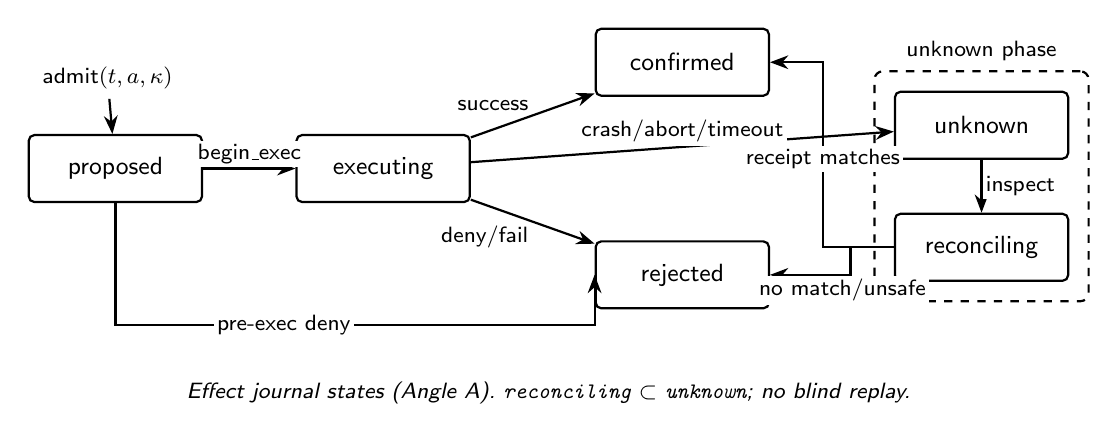
\begin{tikzpicture}[
  font=\sffamily\small,
  >=Stealth,
  state/.style={draw, thick, rounded corners=2pt, align=center,
    minimum width=2.2cm, minimum height=0.85cm, fill=white},
  el/.style={font=\sffamily\footnotesize, fill=white, inner sep=1.2pt}
]
  % Row 1: main happy / deny path
  \node[state] (proposed) at (0,0) {proposed};
  \node[state] (executing) at (3.4,0) {executing};
  \node[state] (confirmed) at (7.2,1.35) {confirmed};
  \node[state] (rejected) at (7.2,-1.35) {rejected};

  % Row right: unknown phase
  \node[state] (unknown) at (11.0,0.55) {unknown};
  \node[state] (reconciling) at (11.0,-1.0) {reconciling};

  \node[draw, thick, dashed, rounded corners=3pt, inner sep=7pt,
        fit=(unknown)(reconciling)] (uphase) {};
  \node[font=\sffamily\footnotesize, anchor=south] at (uphase.north)
    {unknown phase};

  % admit
  \node[font=\sffamily\footnotesize] (admit) at (-0.1,1.15) {admit$(t,a,\kappa)$};
  \draw[thick,->] (admit) -- (proposed);

  \draw[thick,->] (proposed) -- node[el, above] {begin\_exec} (executing);
  \draw[thick,->] (executing) -- node[el, above left] {success} (confirmed);
  \draw[thick,->] (executing) -- node[el, below left] {deny/fail} (rejected);
  \draw[thick,->] (executing) -- node[el, above] {crash/abort/timeout} (unknown);

  \draw[thick,->] (proposed.south) -- ++(0,-1.55) -| (rejected.west)
    node[pos=0.25, el, left] {pre-exec deny};

  \draw[thick,->] (unknown) -- node[el, right] {inspect} (reconciling);
  \draw[thick,->] (reconciling.west) -- ++(-0.9,0) |- (confirmed.east)
    node[pos=0.2, el, above] {receipt matches};
  \draw[thick,->] (reconciling.west) -- ++(-0.55,0) |- (rejected.east)
    node[pos=0.55, el, below] {no match/unsafe};

  \node[font=\sffamily\footnotesize\itshape, align=center]
    at (5.5,-2.85)
    {Effect journal states (Angle~A).
     \texttt{reconciling}~$\subset$~\texttt{unknown}; no blind replay.};
\end{tikzpicture}
\end{document}
